% -*- coding: utf-8 -*-
%-------------------------designed by zcf--------------
\documentclass[UTF8,a4paper,10pt]{ctexart}
\usepackage[left=3.17cm, right=3.17cm, top=2.74cm, bottom=2.74cm]{geometry}
\usepackage{amsmath}
\usepackage{graphicx,subfig}
\usepackage{float}
\usepackage{cite}
\usepackage{caption}
\usepackage{enumerate}
\usepackage{booktabs} %表格
\usepackage{multirow}
\usepackage{pythonhighlight}
\newcommand{\tabincell}[2]{\begin{tabular}{@{}#1@{}}#2\end{tabular}}  %表格强制换行
%-------------------------字体设置--------------
\usepackage{times} 
\newcommand{\yihao}{\fontsize{26pt}{36pt}\selectfont}           % 一号, 1.4 倍行距
\newcommand{\erhao}{\fontsize{22pt}{28pt}\selectfont}          % 二号, 1.25倍行距
\newcommand{\xiaoer}{\fontsize{18pt}{18pt}\selectfont}          % 小二, 单倍行距
\newcommand{\sanhao}{\fontsize{16pt}{24pt}\selectfont}  %三号字
\newcommand{\xiaosan}{\fontsize{15pt}{22pt}\selectfont}        % 小三, 1.5倍行距
\newcommand{\sihao}{\fontsize{14pt}{21pt}\selectfont}            % 四号, 1.5 倍行距
\newcommand{\banxiaosi}{\fontsize{13pt}{19.5pt}\selectfont}    % 半小四, 1.5倍行距
\newcommand{\xiaosi}{\fontsize{12pt}{18pt}\selectfont}            % 小四, 1.5倍行距
\newcommand{\dawuhao}{\fontsize{11pt}{11pt}\selectfont}       % 大五号, 单倍行距
\newcommand{\wuhao}{\fontsize{10.5pt}{15.75pt}\selectfont}    % 五号, 单倍行距
%-------------------------章节名----------------
\usepackage{ctexcap} 
\CTEXsetup[name={,、},number={ \chinese{section}}]{section}
\CTEXsetup[name={(,)},number={\chinese{subsection}}]{subsection}
\CTEXsetup[name={,.},number={\arabic{subsubsection}}]{subsubsection}
%-------------------------页眉页脚--------------
\usepackage{fancyhdr}
\pagestyle{fancy}
\lhead{\kaishu \leftmark}
% \chead{}
\rhead{\kaishu 深度学习及应用作业}%加粗\bfseries 
\lfoot{}
\cfoot{\thepage}
\rfoot{}
\renewcommand{\headrulewidth}{0.1pt}  
\renewcommand{\footrulewidth}{0pt}%去掉横线
\newcommand{\HRule}{\rule{\linewidth}{0.5mm}}%标题横线
\newcommand{\HRulegrossa}{\rule{\linewidth}{1.2mm}}
%-----------------------伪代码------------------
\usepackage{algorithm}  
\usepackage{algorithmicx}  
\usepackage{algpseudocode}  
\floatname{algorithm}{Algorithm}  
\renewcommand{\algorithmicrequire}{\textbf{Input:}}  
\renewcommand{\algorithmicensure}{\textbf{Output:}} 
\usepackage{lipsum}  
\makeatletter
\newenvironment{breakablealgorithm}
  {% \begin{breakablealgorithm}
  \begin{center}
     \refstepcounter{algorithm}% New algorithm
     \hrule height.8pt depth0pt \kern2pt% \@fs@pre for \@fs@ruled
     \renewcommand{\caption}[2][\relax]{% Make a new \caption
      {\raggedright\textbf{\ALG@name~\thealgorithm} ##2\par}%
      \ifx\relax##1\relax % #1 is \relax
         \addcontentsline{loa}{algorithm}{\protect\numberline{\thealgorithm}##2}%
      \else % #1 is not \relax
         \addcontentsline{loa}{algorithm}{\protect\numberline{\thealgorithm}##1}%
      \fi
      \kern2pt\hrule\kern2pt
     }
  }{% \end{breakablealgorithm}
     \kern2pt\hrule\relax% \@fs@post for \@fs@ruled
  \end{center}
  }
\makeatother
%------------------------代码-------------------
\usepackage{xcolor} 
\usepackage{listings} 
\lstset{ 
breaklines,%自动换行
basicstyle=\small,
escapeinside=``,
keywordstyle=\color{ blue!70} \bfseries,
commentstyle=\color{red!50!green!50!blue!50},% 
stringstyle=\ttfamily,% 
extendedchars=false,% 
linewidth=\textwidth,% 
numbers=left,% 
numberstyle=\tiny \color{blue!50},% 
frame=trbl% 
rulesepcolor= \color{ red!20!green!20!blue!20} 
}
%------------超链接----------
\usepackage[colorlinks,linkcolor=black,anchorcolor=blue]{hyperref}
%------------------------TODO-------------------
\usepackage{enumitem,amssymb}
\newlist{todolist}{itemize}{2}
\setlist[todolist]{label=$\square$}
% for check symbol 
\usepackage{pifont}
\newcommand{\cmark}{\ding{51}}%
\newcommand{\xmark}{\ding{55}}%
\newcommand{\done}{\rlap{$\square$}{\raisebox{2pt}{\large\hspace{1pt}\cmark}}\hspace{-2.5pt}}
\newcommand{\wontfix}{\rlap{$\square$}{\large\hspace{1pt}\xmark}}
%------------------------水印-------------------
\usepackage{tikz}
\usepackage{xcolor}
\usepackage{eso-pic}

\newcommand{\watermark}[3]{\AddToShipoutPictureBG{
\parbox[b][\paperheight]{\paperwidth}{
\vfill%
\centering%
\tikz[remember picture, overlay]%
  \node [rotate = #1, scale = #2] at (current page.center)%
    {\textcolor{gray!80!cyan!30!magenta!30}{#3}};
\vfill}}}



%———————————————————————————————————————————正文———————————————————————————————————————————————
%----------------------------------------------
\begin{document}
\begin{titlepage}
    \begin{center}
    
\includegraphics[width=0.8\textwidth]{NKU.png}\\[1cm]    
    \textsc{\Huge \kaishu{\textbf{南\ \ \ \ \ \ 开\ \ \ \ \ \ 大\ \ \ \ \ \ 学}} }\\[0.9cm]
    \textsc{\huge \kaishu{\textbf{计\ \ 算\ \ 机\ \ 学\ \ 院}}}\\[0.5cm]
    \textsc{\Large \textbf{深度学习及应用实验作业}}\\[0.8cm]
    \HRule \\[0.9cm]
    { \LARGE \bfseries 作业三 \  生成对抗网络实践}\\[0.4cm]
    \HRule \\[2.0cm]
    \centering
    \textsc{\LARGE \kaishu{姓名\ :\ 王泳鑫}}\\[0.5cm]
    \textsc{\LARGE \kaishu{学号\ :\ 1911479}}\\[0.5cm]
    \textsc{\LARGE \kaishu{年级\ :\ 2019级}}\\[0.5cm]
    \textsc{\LARGE \kaishu{专业\ :\ 计算机科学与技术}}\\[0.5cm]
    \textsc{\LARGE \kaishu{指导教师\ :\ 侯淇彬}}\\[0.5cm]
    \vfill
    {\Large \today}
    \end{center}
\end{titlepage}
%-------------摘------要--------------
\newpage
\thispagestyle{empty}
\renewcommand{\abstractname}{\kaishu \sihao \textbf{摘要}}
    \begin{abstract}
        本次实验基于FashionMNIST数据集进行实践。
        \noindent  %顶格
        \textbf{\\\ 关键字:前馈神经网络,pytorch,FNN}\textbf{} \\\ \\\
    \end{abstract}
%----------------------------------------------------------------
\tableofcontents
%----------------------------------------------------------------
\newpage
\watermark{60}{10}{NKU}
\setcounter{page}{1}
%——————————————————————————————————————


\section{实验要求}

\begin{itemize}
    \item 掌握GAN原理
    \item 学会使用PyTorch搭建GAN网络来训练FashionMNIST数据集
\end{itemize}


\section{GAN网络结构}

如图\ref{fig:1}所示
\begin{figure}[H]
    \centering
    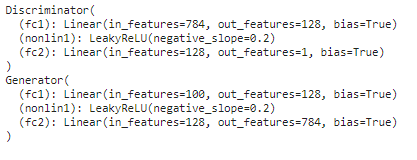
\includegraphics[scale=1]{1.png}
    \caption{Caption}
    \label{fig:1}
\end{figure}

\section{loss曲线}

如图\ref{fig:1}所示
\begin{figure}[H]
    \centering
    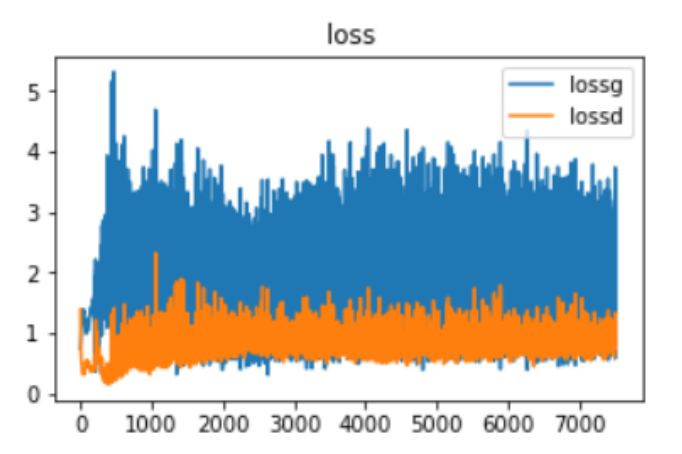
\includegraphics[scale=0.5]{2.png}
    \caption{Caption}
    \label{fig:1}
\end{figure}


\section{随机数生成图}

\begin{python}
    f = torch.randn(8,100,device=device)
    x = G(f)
    show_imgs(x)

\end{python}

生成结果如图\ref{fig:1}所示
\begin{figure}[H]
    \centering
    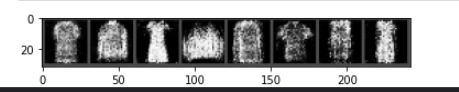
\includegraphics[scale=0.5]{3.png}
    \caption{Caption}
    \label{fig:1}
\end{figure}


针对自定义的 100 个随机数,自由挑选 5 个随机数,查看调整每个随机数时,生成图像
的变化(每个随机数调整 3 次,共生成 15x8 张图),总结调整每个随机数时,生成图像
发生的变化。





\subsection{修改一}

修改第二个随机数为 0,10,100,如下图(从上到下依次为 未修改原图,0,10,
100),生成结果如图\ref{fig:1}所示
\begin{figure}[H]
    \centering
    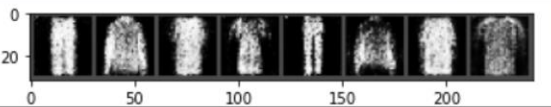
\includegraphics[scale=0.5]{4.png}
    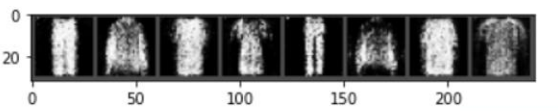
\includegraphics[scale=0.5]{5.png}
    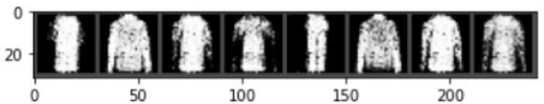
\includegraphics[scale=0.5]{6.png}
    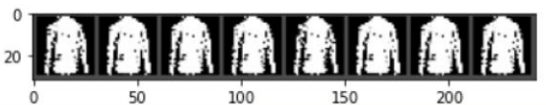
\includegraphics[scale=0.5]{7.png}
    \caption{Caption}
    \label{fig:1}
\end{figure}


发现随着第二个随机数的增大,长袖上衣的图像越来越明显,说明第二个随机数与
此类分布关系紧密。




\subsection{修改二}

修改第七十一个随机数为-10,10,100,如下图(从上到下依次为 -10,原图,10,
100),生成结果如图\ref{fig:1}所示
\begin{figure}[H]
    \centering
    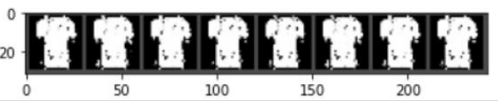
\includegraphics[scale=0.5]{8.png}
    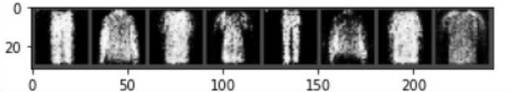
\includegraphics[scale=0.5]{9.png}
    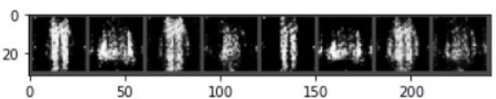
\includegraphics[scale=0.5]{10.png}
    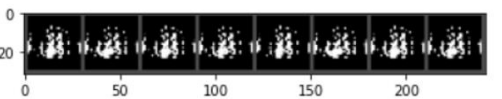
\includegraphics[scale=0.5]{11.png}
    \caption{Caption}
    \label{fig:1}
\end{figure}

可以看到,随着第 71 个随机数的减小,白色短袖轮廓特征的图像越来越明显,随
着该随机数的增大,轮廓越来越不明显。



\subsection{修改三}
修改第一百个随机数为-50,-10,10,如下图(从上到下依次为 10,原图,-10,
-50),生成结果如图\ref{fig:1}所示
\begin{figure}[H]
    \centering
    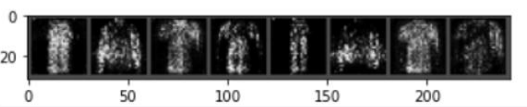
\includegraphics[scale=0.5]{12.png}
    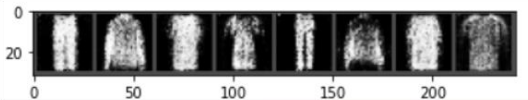
\includegraphics[scale=0.5]{13.png}
    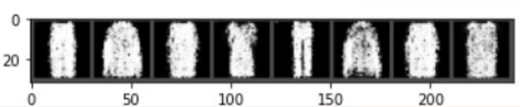
\includegraphics[scale=0.5]{14.png}
    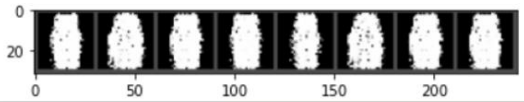
\includegraphics[scale=0.5]{15.png}
    \caption{Caption}
    \label{fig:1}
\end{figure}

可以看到,随着第 100 个随机数的减小,白色长方体越来越明显,随着该随机数的
减小,该特征越来越不明显,导致几乎所有图片越来越黑.



%----------------------------------------------------------------

%----------------------------------------------------------------
\bibliographystyle{plain}
\end{document}
